%<*standalone>
\documentclass{standalone}

\usepackage{tikz}
\usetikzlibrary{calc}
\newsavebox\mybox

\begin{document}
%</standalone>
% Diagram of the TeX box model and its dimensions
% Copyright (C) 2001 by Martin Scharrer <martin@scharrer.me>, Nov 12th 2011
% This is free code under the LPPL v1.3 or later version OR the CC BY-SA 3.0
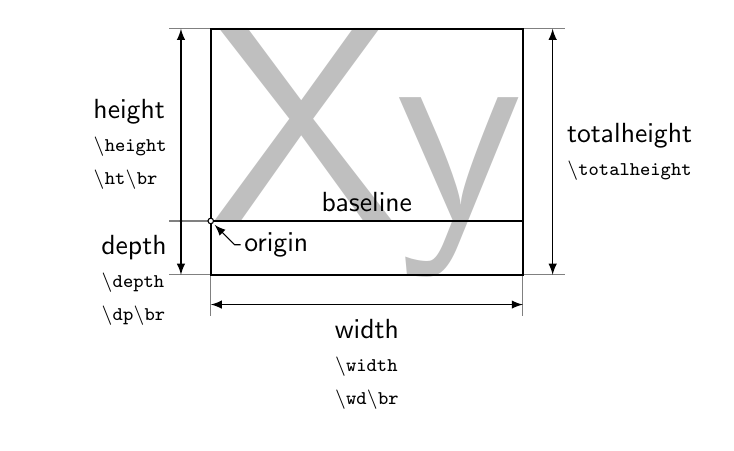
\begin{tikzpicture}[font=\sffamily,>=latex]
   \newcommand\Cs[1]{\texttt{\scriptsize\textbackslash #1}}
% Save example text in box
   \sbox\mybox{\pgfinterruptpicture\sffamily\color{black!25}\scalebox{10}{Xy}\endpgfinterruptpicture}
   \def\HEIGHT{\ht\mybox}
   \def\WIDTH{\wd\mybox}
   \def\DEPTH{\dp\mybox}
% Extensions lines for dimensions (drawn here to be below other material)
   \draw [gray,thin]
        (0,0)            -- +(-3.5ex,0)
        (0,\HEIGHT)      -- +(-3.5ex,0)
        (0,-\DEPTH)      -- +(-3.5ex,0)
        (\WIDTH,\HEIGHT) -- +(3.5ex,0)
        (\WIDTH,-\DEPTH) -- +(3.5ex,0)
        (0,-\DEPTH)      -- +(0,-3.5ex)
        (\WIDTH,-\DEPTH) -- +(0,-3.5ex)
   ;
% Text node:
   \node [inner sep=0pt,anchor=base west] {\usebox\mybox};
% Baseline
   \draw (0,0) -- (\WIDTH,0) node [above,midway] {baseline};
% Box
   \draw [thick] (0,-\DEPTH) rectangle (\WIDTH,\HEIGHT);
% Origin
   \path [fill=white,draw=black] (0,0) circle (1pt);
   \draw [<-,shorten <=2pt] (0,0) -- (2ex,-2ex) -- +(.5ex,0) node [right=-0.5ex] {origin};
% Dimensions
   \tikzset{inner sep=5pt}
   \draw [->] (-2.5ex,0) -- +(0,-\DEPTH)  node [pos=1.1,left,align=left]
        {depth\\\Cs{depth}\\\Cs{dp}\Cs{br}};
   \draw [->] (-2.5ex,0) -- +(0, \HEIGHT) node [pos=.4,left,align=left]
        {height\\\Cs{height}\\\Cs{ht}\Cs{br}};
   \draw [<->] (\WIDTH,-\DEPTH) ++(2.5ex,0) -- +(0,\DEPTH+\HEIGHT) node [midway,right,align=left]
        {totalheight\\\Cs{totalheight}};
   \draw [<->] (0,-\DEPTH) ++(0,-2.5ex) -- +(\WIDTH,0) node [midway,below,align=left]
        {width\\\Cs{width}\\\Cs{wd}\Cs{br}};
   \fill (-2.5ex,0) circle (.5pt);
% Center inner box
   \path let
        \p1 = (current bounding box.south west),
        \p2 = (current bounding box.north east),
        \p3 = (0,-\DEPTH),
        \p4 = (\WIDTH,\HEIGHT)
   in
        (\x3-\x2+\x4,\y3) rectangle (\x4+\x3-\x1,\y4);
\end{tikzpicture}
%<*standalone>
\end{document}
%</standalone>
